\section{Clustering}\label{bg:clustering}\note{Should maybe be moved to description of collaborative filtering}
Clustering is a widely used method when working with a large amount of data. In short it is about grouping similar data in ``clusters''. In the domain of recommending clustering is commonly used together with the recommendation method called collaborative filtering, where the data is clustered into users with similar ratings for given items. The user data in these clusters are then used to make individual recommendations to the users.

One of the most efficient collaborative filtering methods which uses clustering is matrix factorization, described in \sectionref{bg:matrixfactorization}. 

Looking at the dataset we get when we have to make group recommendations, it is rather small compared to what is used in normal group recommenders.

Although using clustering in general give some good results, clustering when recommending to groups is not the most suitable solution, unless the group members are compared to a large database of users, where clustering becomes a decent if not great method to improve the execution time of the comparison.

%\begin{figure}[H]
%	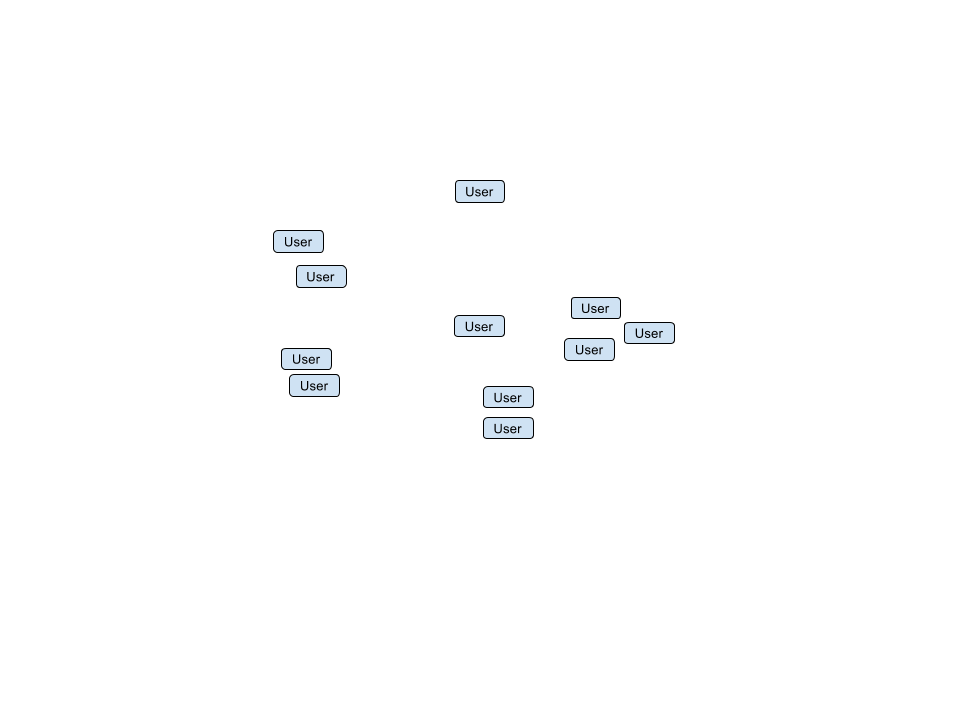
\includegraphics[scale=1]{graphics/Clustering_1.png}
%\end{figure}

%When using clustering for recommendation systems typically they are used in collaborative filtering to find users with similar interests and predict new items based on users in the same clusters.


